\section{Theorie}
\subsection{Grundlagen}
Zur Untersuchung mittels Tomographie wird das Objekt, das untersucht werden soll, mit Strahlung durchdrungen.
Bei dieser Strahlung kann es sich, je nach zu untersuchendem Körper, um Teilchenstrahlung oder um radioaktive Strahlung handeln.
Durch die Abschwächung, die der Strahl durch das Durchdringen erfährt, kann über die gemessene Intensität auf die Materialeigenschaft rückgeschlossen werden.
Wenn das Objekt von unterschiedlichen Seiten bestrahlt wird, lässt sich so ein räumliches Bild erstellen.
In diesem Versuch wird als $\gamma$-Strahlungsquelle $\ce{^{137}Cs}$ verwendet. Es zerfällt zu $\ce{^{137}Ba}$.
Mit einer Wahrscheinlichkeit von $6,5 \%$ zerfällt es direkt in den Grundzustand.
Zum größten Teil aber, zerfällt es in einen angeregten Bariumkern, der unter Aussendung eines Photons schließlich auch in den Grundzustand fällt.

\begin{figure}[H]
  \centering
  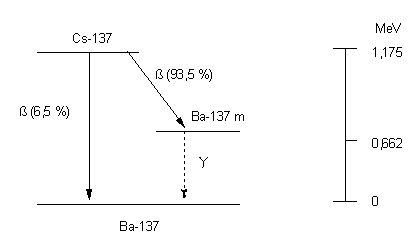
\includegraphics[width=0.7\textwidth]{Bilder/caesium.png}
  \caption{Zerfall von $\ce{^{137}Cs}$.\cite{caesium}}
  \label{fig:caesium}
\end{figure}

Die Strahlung wechselwirkt unter drei Prozessen mit Materie.
Beginnend mit dem Photoeffekt, der erst auftritt, wenn die Energie des Lichtteilchens größer als die Bindungsenergie eines Elektrons ist, wird ein Elektron der Hülle eines
Atoms durch auftreffende Photonen aus seiner Bindung herausgeschlagen.
Der nächste Effekt ist der Compton-Effekt, der mit einer Photonenenergie zwischen $100\, \si{keV}$ und $10\, \si{MeV}$ dominiert.
Er bezeichnet die Vergrößerung der Wellenlänge eines auf ein Elektron treffendes Photon.\\
Das Photon wird im Gegensatz zum Photoeffekt nicht vollkommen absorbiert, sondern nur am Elektron gestreut. Dabei ist die Zunahme der Wellenlänge des Photons
abhängig zum Streuwinkel.\\
Zuletzt versteht man unter Paarbildung den Zerfall eines Photons im Coulomb-Feld eines Atomkerns.
Es entsteht ein Elektron-Positron-Paar, sodass die Energie des Photons mindestens der Ruheenergie eines Elektrons und eines Positrons entsprechen muss.
Dies ist bei einer Energie von $2m_ec^2 = 1,02\, \si{MeV}$ der Fall.
Da in diesem Versuch eine $\ce{^{137}Cs}$ Quelle verwendet wird, ist dieser Prozess energetisch bedingt nicht von Bedeutung.

\subsection{Bestimmung des Absorptionskoeffizienten}
Jedes Material ist durch seinen Absorptionskoeffizienten $\mu_i$ charakterisiert.
Um mithilfe der Tomographie auf ein Element zurückzuschließen, muss dieser also bestimmt werden.
Insgesamt gilt ein Zusammenhang
\begin{equation}
  N=I_0 \exp \Bigl(\sum_{i}\mu_i d_i\Bigr)
\end{equation}
zwischen der Intensität $N$ und dem Absorptionskoeffizienten $\mu$, der Eingangsintensität $I_0$ sowie der Wegstrecke $d$, die der Strahl innerhalb des Würfels zurücklegt.
Für die j-te Projektion folgt somit
\begin{equation}
  \sum_{i}\mu_i d_i =\ln \Bigl(\frac{I_0}{N_j}\Bigr).
\end{equation}
Durch Messen der einzelnen Schichten lassen sich durch Lösen des Gleichungssystems die Zusammensetzung dieser und somit der einzelnen Würfelelemente bestimmen.
Durch mehrmaliges Messen wird das Gleichungssystem überbestimmt und somit die Genauigkeit erhöht.
Im Generellen wird die Gleichung
\begin{equation}
  A \mu = I
  \label{eq:matrix}
\end{equation}
gelöst.
Durch die Methode der kleinsten Quadrate wird die Matrixgleichung $\ref{eq:matrix}$ in die Normalengleichung
\begin{equation}
  (A^TA)\mu = (A^T I)
\end{equation}
umgeschrieben.
Umgestellt nach dem jeweiligen Absorptionskoeffizienten folgt schließlich
\begin{equation}
  \mu = (A^T A)^\text{-1}A^TI.
\end{equation}
Vereinfacht für alle Raumrichtungen folgt für die Abweichung $\sigma_i^2$ von $\mu_i$ aus dem ersten Diagonalelement
\begin{equation}
  C=\sigma_I^2(A^TA)^\text{-1}.
  \label{eq:abweichung}
\end{equation}
\clearpage
